This option allows users to generate synthetic ground motions for a
target seismic event. In order to do so, the stochastic ground motion
model is selected from the drop-down menu, as shown
in \Cref{fig:stochastic_loading}. Depending on the model selected, the
user will be asked to enter values for a number of parameters that are
used to generate a seismic event. In the current release, users can
select between the model derived by Vlachos et
al. (2018) \cite{vlachos2018predictive} and the model developed by
Dabaghi \& Der Kiureghian (2014, 2017, 2018)
[\cite{dabaghi2014stochastic}, \cite{dabaghi2017stochastic}, \cite{dabaghi2018simulation}]. The
geometric directivity parameters, as shown in \Cref{fig:dabaghi}, required by the Dabaghi \& Der
Kiureghian model are described completely in Somerville et al. (1997)
\cite{somerville1997modification}. Additionally, users can provide a
seed for the stochastic motion generation if they desire the same
suite of synthetic motions to be generated on multiple occasions.  If
the seed is not specified, a different realization of the time history
will be generated for each run. The backend application that generates
the stochastic ground motions relies on \texttt{smelt}, a modular and
extensible C++ library for generating stochastic time histories. Users
interested in learning more about the implementation and design of
\texttt{smelt} are referred to its
\href{https://github.com/NHERI-SimCenter/smelt}{GitHub repository}.

All input parameters can be specified as random variables by entering
a string in the parameter field. Please note that information for the
inputs that are identified as random variables needs to be provided in
the \texttt{UQ} tab.

\begin{figure}[!htbp]
  \centering
    \begin{subfigure}{\textwidth}
        \centering
        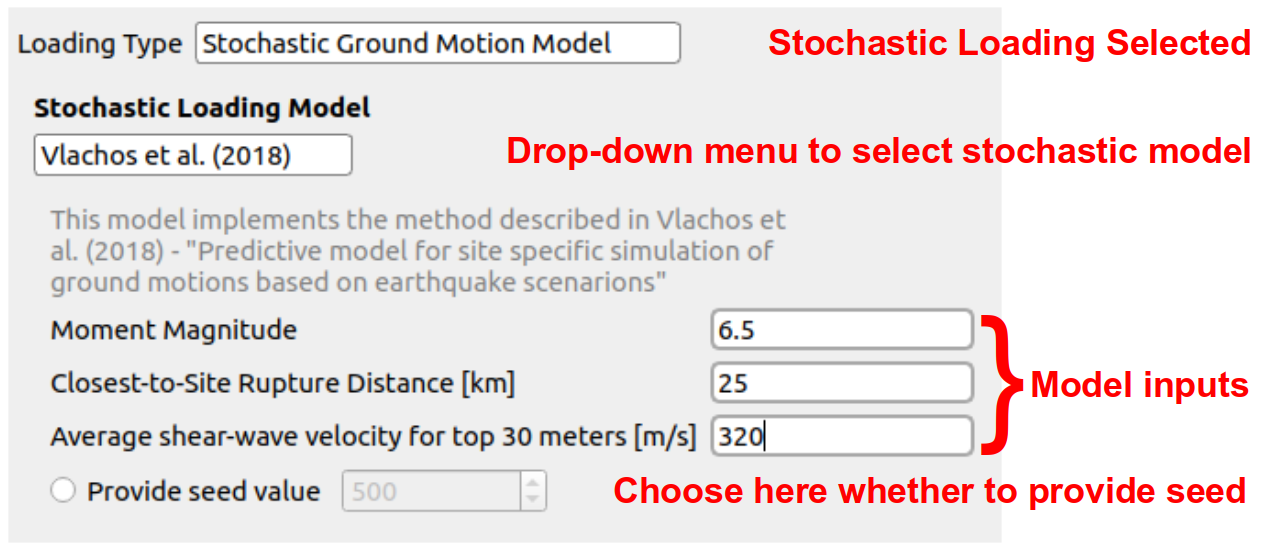
\includegraphics[width=\textwidth]{usage/figures/stochastic_loading.png}
        \caption{Vlachos et al. (2018) model inputs}
    \end{subfigure}
    \hspace*{\fill}
    
    \begin{subfigure}{\textwidth}
        \centering
        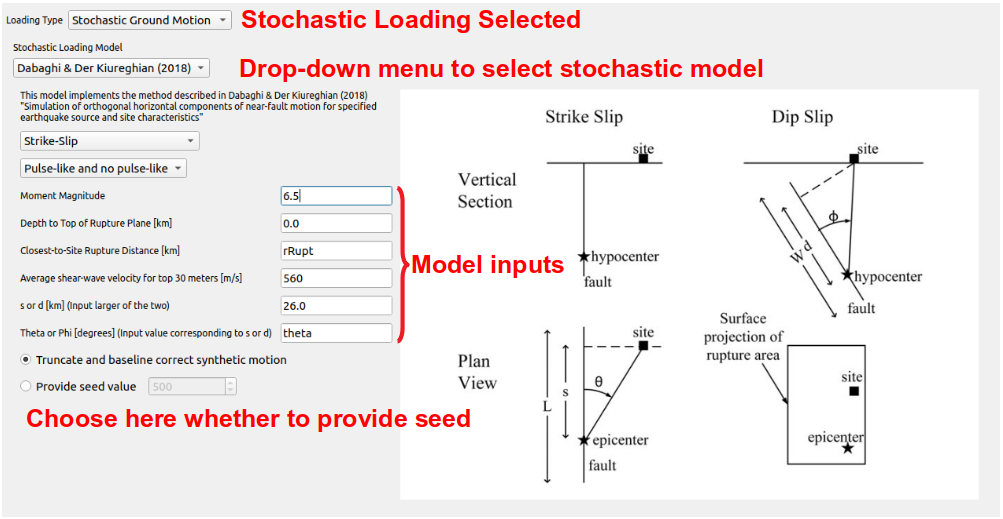
\includegraphics[width=\textwidth]{usage/figures/stochastic_dabaghi.png}
        \caption{Dabaghi \& Der Kiureghian (2018) model inputs}
        \label{fig:dabaghi}        
    \end{subfigure}
    
  \caption{Stochastic Ground Motion Event}
  \label{fig:stochastic_loading}    
\end{figure}
